\section{Introduction}
Due to Zynq's unique advantages such as being reconfigurable and low power consumption, various deep learning and acceleration work based on the embedded terminal have been conducted on various in-depth researches based on the platform.

In terms of neural network computing architecture, Zhang\cite{zhang2015optimizing} proposed a Roofline method for analyzing overall throughput to obtain the architecture with the best performance and the lowest FPGA resource and parallelism. To optimization the memory access, Shen\cite{ma2017hardware} presented a flexible data buffer solution to ensure the balance between input and weight transmission bandwidth, significantly reduced the memory access for the convolution accelerator, Manoj Alwani\cite{alwani2016fused} presented a by modifying and fusion among layers of data types and enable the sequence of input data on the chip, and through the model evaluation of the data on the intermediate results. In terms of matrix fast multiplication, Liang\cite{lu2017evaluating} proposed a compute architecture using Winograd algorithm to realize convolution neural network, and adopted the row buffer structure to effectively reuse the characteristics between different data blocks, so as to improve the final running speed. In terms of neural network model compression, Han\cite{han2015deep} designed a quantitative pruning method based on neural network model to reduce the weight and the number of calculates for neural network.

The research for deep learning acceleration based on embedded platform from different aspects, such as Fast matrix multiplication algorithm ,Compression and computing structure plays a role of promotion,but the bulk of the research is not open source,  It makes further researchers need to spend time cost on the basis of existing research, rather than on further innovation work.

At present , the research and application for deep learning based on Zynq platform have some deficiencies:it need developers are familiar with the deep learning algorithm and the hardware and software system, the Zynq platform using the threshold is high, causes the limited depth of developers, affected the Zynq with the depth study of large-scale embedded applications.therefore Xilinx create Pynq project, support Python in deep learning algorithm research at embedded platform, hoping to expand user numbers.

Pynq is a developed platform for developing software with Python to accelerate the AI algorithms. It supports the use and development of various Python algorithms library, so that developers and researchers can focus more on the application of software algorithms rather than the development of the underlying hardware. Pynq purpose is through to the Python language support, expand the number of users on Zynq system, but based on Pynq,AI research of accelerating there are design elements, the research process is difficult, the workload is relatively cumbersome, to physical, from obtaining and using the Python language until the underlying hardware, models, diversity and accuracy, framework and the corresponding fixed-point quantitative tool use, overall demand by the tool resources and computing resources scattered and time-consuming, cause contribution has been not effectively improve the number of developers.

In order to solve the above problems, this paper proposes to set up a comprehensive platform to integrate all the elements involved in the research at the same platform. Researchers only need to connect to the Internet to conduct deep learning acceleration research based on Pynq.

\begin{figure}
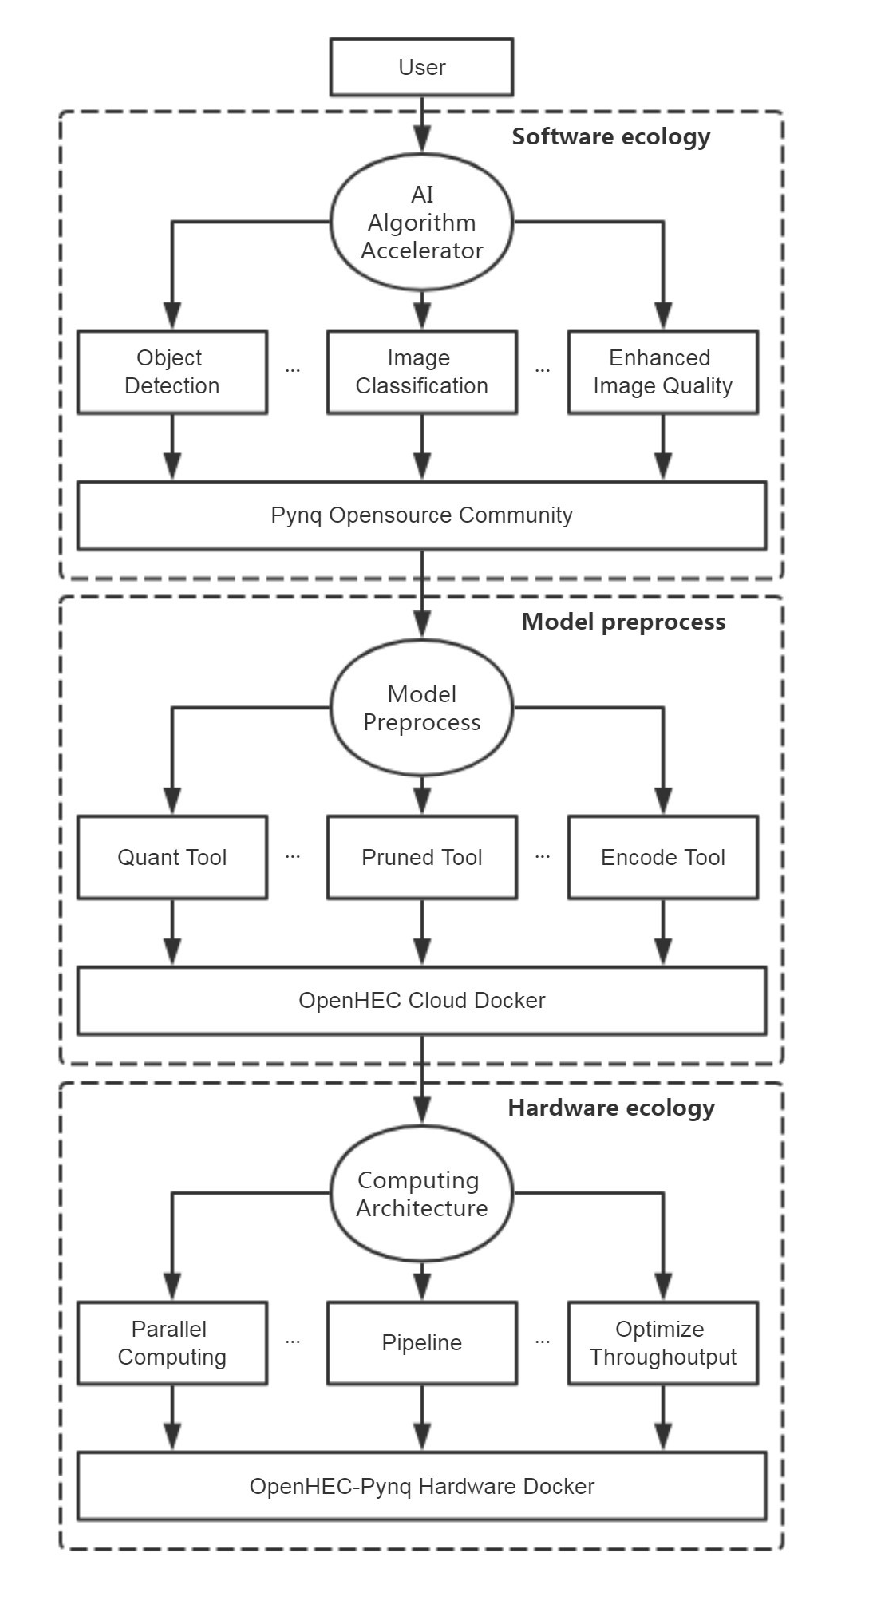
\includegraphics[height=7.2in, width=3.6in]{figure_0}
\caption{XXX}
\end{figure}

The main work of this paper is as follows:
\begin{enumerate}
    \item model quantification tools required under different deep learning frameworks, official data sets required by model training, vivado-hls development tool chain, and integration of different deep learning frameworks.
    \item With Pynq and other original Zynq series FPGA embedded platforms, virtual dynamic mapping will be carried out in the cloud for user development and research.
    \item Taking YOLOv2, the current mainstream deep-learning target detection algorithm, as an example, we demonstrate the research on the FPGA cloud hardware platform by using pynq-based deep learning acceleration tool.
\end{enumerate}

\section{Elements involved in AI development - based Pynq}
The development of the embedded platform based on Pynq requires a lot of basic knowledge of software and hardware to integrate with the overall knowledge elements. After obtaining the model, a large number of labeled data sets are required to train the network model, The official data sets are complex and the model transformation under the framework of various neural networks is also difficult.

\begin{figure*}
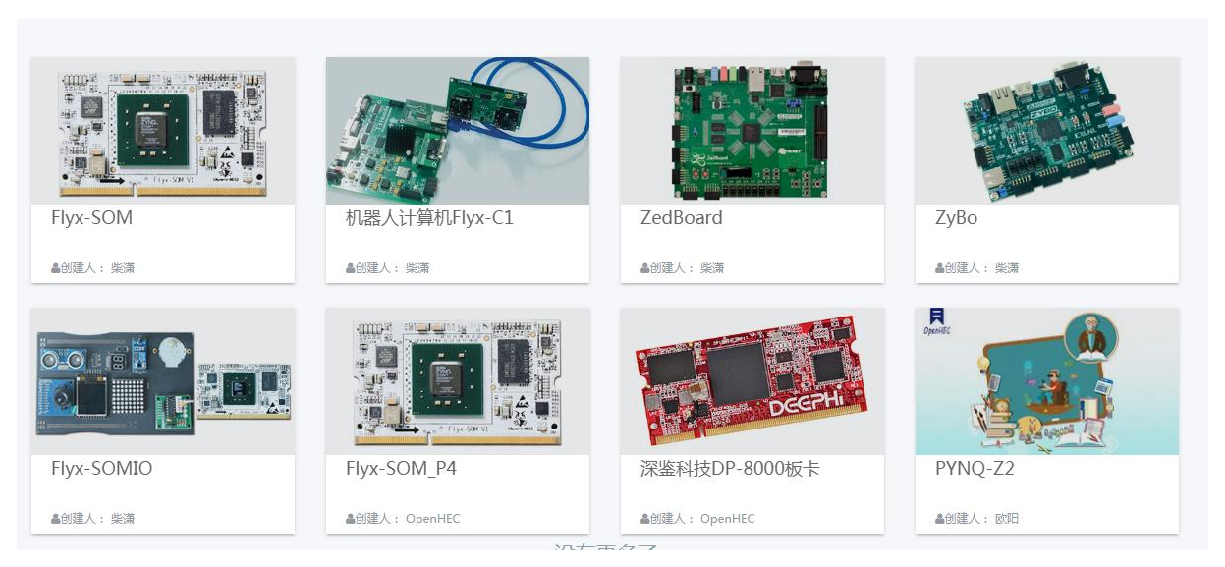
\includegraphics[height=3in, width=6in]{figure_1}
\caption{A sample black and white graphic.}
\end{figure*}

\subsection{Official datasets}
The official data set required by the research direction of neural network, such as the COCO data set of target detection,Professional data sets such as ImageNet data sets of picture classification. And target detection COCO data set.

Target detection COCO data set is Microsoft's team to establish a subtitles can be used to identify, segmentation, image data sets, the data sets to scene understanding as the goal, mainly from the complex daily interception in the scene, the image of target position by accurate segmentation of calibration. Images include class 91 targets, 328,000 images and 2,500,000 labels.

ImageNet is the first large-scale image data set introduced in 2010; The data set was stable in 2012. It contains an image of 1000 classes. The ImageNet category has a hierarchy. Select 1000 classes so that there is no overlap in the ImageNet hierarchy. And the ImageNet dataset contains many fine-grained categories, including 120 different breeds of dogs. There are 13,000 training images (732 to 1,300 per class), 100,000 test images (100 per class) and 50,000 verified images (50 per class). The ImageNet challenge accuracy report USES two metrics :top 5 and top 1 errors. A top-five error means that if any of the top five is correct, it is considered a proper classification. The top 1 items requiring the highest scores are correct.

\subsection{Fixed-point quantitative open source tools}
At present, there are three kinds of fixed-point tools for floating-point model, which are low-number floating-point approximation, dynamic fixed-point approximation and weighting exponential fixed-point approximation.

\subsubsection{Low bit wide floating point approximation representation}
The low point wide floating point number approximation completely conforms to the IEEE754 floating point number representation standard, and the low point wide floating point accuracy is used to approximate the high point wide floating point data. In addition to reducing the model size, this method generally uses floating point number calculation, which has little effect on the precision, and it does not help the hardware developers to improve the calculation speed.

\subsubsection{Low bit wide floating point approximation representation}
The low point wide floating point number approximation completely conforms to the IEEE754 floating point number representation standard, and the low point wide floating point accuracy is used to approximate the high point wide floating point data. In addition to reducing the model size, this method generally uses floating point number calculation, which has little effect on the precision, and it does not help the hardware developers to improve the calculation speed.

\subsubsection{Dynamic fixed point accuracy quantification}
Each number n of dynamic fixed-point precision quantification represents the specific process as shown in formula 1:
\begin{equation}
  n = (-1)^s * 2^{-fl} * \sum_{i=0}^{B-2} 2^i * x_i
\end{equation}
B here is a bit wide, s is the sign bit, f1 is fractions length, x is the mantissa, n actual values, by dynamic fixed-point quantitative floating point precision fitting model, through the determination of each layer of fixed-point different fixed-point allocation, each network layer can be divided into three groups: one for the input layer, one for the weight, one for the output layer, it can better cover the dynamic range of activation and weights.

\subsubsection{weight exponential}
Convolution multiplication is replaced by Left shift operator and Right shift operator. The fully connected layer and convolution layer are composed of increasing and multiplying, where the multiplier requires more chip area. This prompted previous studies to eliminate all multipliers by using integer weights shift operator. These weights can be thought of as minifloat Numbers with zero mantissa. The multiplication between the weights and the layer activation becomes displacement, the weight exponential represents the specific process as shown in formula (2), s is the sign bit ,exp is the power of the fixed point data.
\begin{equation}
  n = (-1)^s * 2^{exp}
\end{equation}

\subsection{Vivado-HLS development tool chain}
Vivado-HLS tool chain for Xilinx FPGA hardware logic development tools, developers use the development tool chain for hardware logic description.

\subsection{Virtualized Pynq cloud hardware platform}
Multi-block Pynq cloud sharing by providing network nodes for users to verify current research results.

At present, hardware developers usually study the computing architecture of AI algorithm by using all the above development elements. However, it will take a lot of time for them to collect all the elements for research. Therefore, it is vital to build a platform integrating all elements both and software and hardware for the development and research of neural network algorithm.

\section{AI open source platform architecture based on Pynq}

\subsection{Ideal architecture}
The ideal architecture display on Figure 0.The developer uploads the model to the cloud platform, and calls the framework and data set owned by the cloud platform to train and test the network model. Developers can then use the tools provided by the platform to quantify the model and perform hardware design and optimization on the cropped network.

\subsection{Hardware cloud platform}
The open source cloud hardware platform saves developer time cost by integrating research elements. The open source tool and implementation code allow developers to conduct multi-scale and multi-level research based on Pynq deep learning acceleration.Display on Figure 1.

\subsection{Tool integration}
The floating-point operation in the AI algorithm will consume a lot of resources in the hardware design. Due to the robustness of the algorithm itself \cite{courbariaux2014low}, fixed-point operations can be used instead of floating-point operations under the condition of ensuring less loss of precision or even lossless. At present, such methods have become one of the main steps of current hardware acceleration. Therefore, the platform also integrates a variety of quantitative tools under the neural network framework, which greatly reduces the time cost for researchers to find quantitative algorithms and tools.

\section{Openhec-Pynq}
The cloud platform is equipped with the Darknet framework, in which we analyzes the YOLOv2 network structure, extracts the required parameters and weights of each layer, and writes the C Model for HLS.

In addition, since reference \cite{qiu2016going, shan2016dynamic} has shown that low-precision quantization is sufficient for CNN implementation, in addition to using 32-bit to represent intermediate results, 16-bit fixed-point are used for input data, weights, and output data.

After verification by software simulation, the HLS-based accelerator design and optimization are performed. Finally, we implemented control and communication for the HLS-based YOLOv2 accelerator through Python for easy use on the Pynq platform.

\subsection{Design and Optimization of YOLOv2 Accelerator Based on FPGA}
According to the analysis of the YOLOv2 network, most layers are serially processed, except for the routing layer. The routing layer can be implemented by setting a specific address in advance. 

From an accelerator perspective, the work required is to interact with memory in order (reading memory data, processing data, and then writing back memory data). Since the amount of data input and output is very large, loop tiling technique is always applied to reuse data and reduce memory access times, which tiles the convolution loop R, C, M, N to Tr, Tc, Tm ,Tn\cite{zhang2015optimizing}.

The overall architecture of the accelerator is shown below:

\begin{figure}
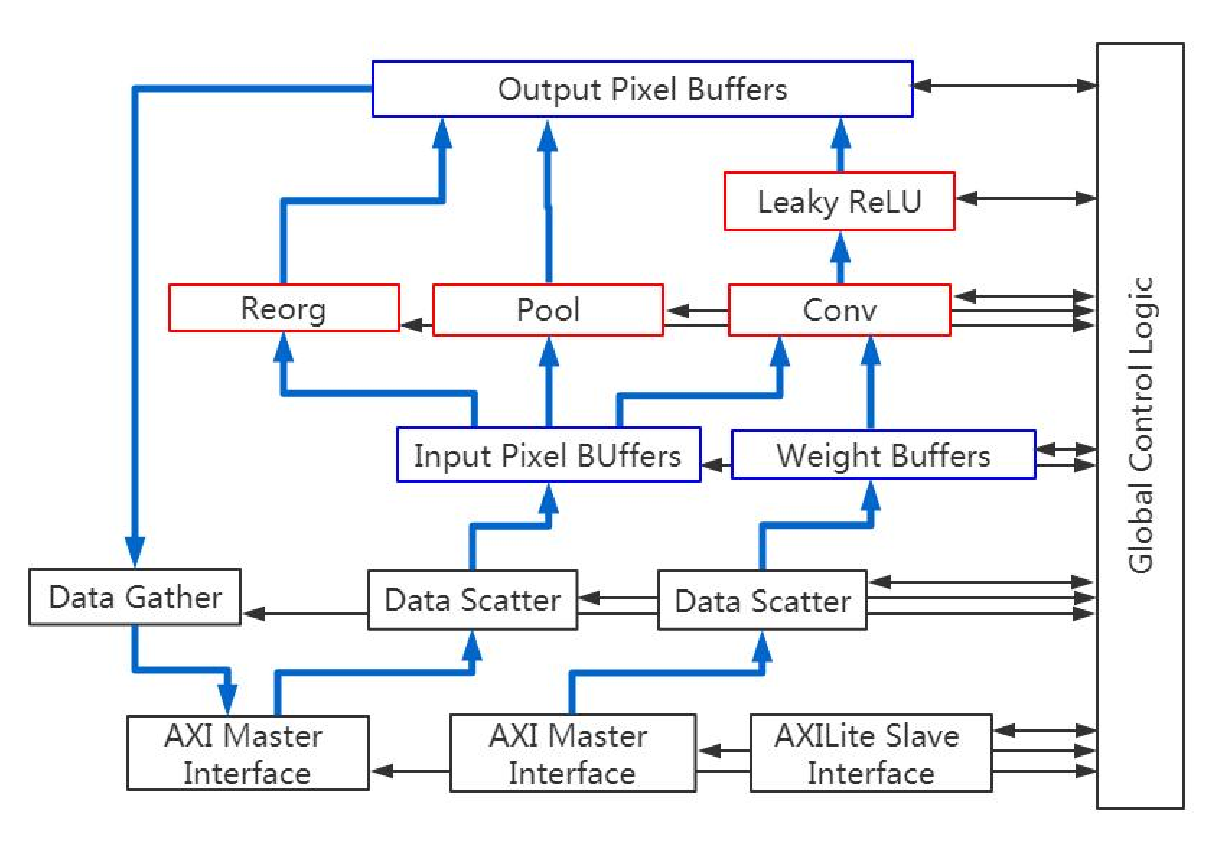
\includegraphics[height=3.1in, width=3.6in]{figure_2}
\caption{XXX}
\end{figure}

Similar to \cite{zhang2015optimizing, chen2014diannao, ma2017automatic}, the accelerator has two AXI4 master interfaces and one AXI4-Lite slave interface. AXI-Lite slave interface is responsible for reading and writing control, data and status register sets. The input feature maps and weights are read concurrently by two master interfaces, and the output feature maps are written back simultaneously through write channel. 

The Data Scatter module is designed to generate the corresponding write address and distribute the data read from the DRAM to the on-chip buffers. The Data Gather module is designed to generate the DRAM write-back address and write the data in the output buffer back to the DRAM. The other red modules are responsible for the processing of the convolutional layer (Conv and Leaky ReLU), the maximum pooling layer (Pool) and the reorg layer (Reorg).

\begin{table*}
  \caption{Frequency of Special Characters}
  \label{tab:freq}
  \begin{tabular}{cccccc}
    \toprule
    {\quad}&DSP&BRAM&LUT&FF&Freq\\
    \midrule
    Fixed-16 & 106(48\%) & 100(72\%) & 27495(52\%) & 30118(28\%) & 130MHz\\
    Float-32 & 207(94\%) & 120(86\%) & 27816(52\%) & 27816(26\%) & 100MHz\\
  \bottomrule
\end{tabular}
\end{table*}

\begin{table*}
  \caption{Some Typical Commands}
  \label{tab:commands}
  \begin{tabular}{cccccc}
    \toprule
    {\quad}& \cite{ma2017hardware} & \cite{venieris2016fpgaconvnet}& \cite{wang2018pynq}&Ours&Ours\\
    \midrule
    CNN models & Tiny-YOLO v1& Scene Labelling&LeNet-5&YOLO v2&YOLO v2 \\
    FPGA Board(FPGA) & VC707(Virtex7 485t) & Zedboard(XC7Z020) & Pynq(XC7Z020) & Pynq(XC7Z020)& Pynq(XC7Z020)\\
    Clock(MHz) & 143 & 100 & 100 & 100 & 130\\
    Precision & Fixed-16 & Fixed-16 & Fixed-8 & Float-32 & Fixed-16\\
    Power(W) & - & - & - & 2.39 & 2.71\\
    Operations(GOP) & 3.09 & - & $4.58*10^{-3}$ & 29.47 & 29.47\\
    Performance(GOP/s) & 64.86 & 12.73 & 2.56 & 2.53 & 11.39\\
    Power Efficiency(GOP/s/W) & - & 7.27 & 1.35 & 1.06 & 4.20\\
    \bottomrule
  \end{tabular}
\end{table*}

\subsubsection{Weight Arrangement}
The effective FPGA bandwidth goes up with the increase of burst length and finally flattens out above some burst length threshold\cite{zhang2016caffeine}. The data tiling technique usually results in a discontinuous DRAM access for the row-major data layout in DRAM. To reduce the number of memory accesses and increase the effective memory bandwidth, we arrange the kernel weights for an entire tile to a continuous block to ensure a high utilization of the bandwidth of external memory \cite{qiu2016going}.

\subsubsection{Parallel Convolution Engine}
The acceleration strategy of convolutional layer is similar to \cite{zhang2015optimizing, motamedi2017placid}, which utilizes input and output parallelism to accelerate the computation. By designing multiple parallel multiplication units and add trees to achieve input parallelism (Tn parallelism) and output parallelism (Tm parallelism) in convolution calculation. The Tm*Tn multiplication units are calculated in parallel. The add trees of Log2 (Tn) depth are accumulated by pipeline, and generate the partial sums.

\subsubsection{Ping-Pong operation}
Similar to \cite{zhang2015optimizing}, the design implements ping-pong buffers to overlap the delay of reading input feature maps and weights, writing output feature maps and calculation, which greatly improves the dynamic utilization of the computing engines.

\section{Comparison}
Two data precision types of float32 and dynamic fixed-point 16-bit have been designed. Experiments show that floating point addition in HLS requires three DSP resources, floating point multiplication requires two DSPs; fixed point 16-bit multiplication requires one DSP, and fixed-point 16-bit addition can be implemented only using LUT. After placing and routing, resource consumptions of float32 (Tn=3, Tm=9, Tr=26, Tc=52) and fixed-16 (Tn=2, Tm=32, Tr=26, Tc=26) are shown as table 1.

According to the current design, DSP and BRAM are more expensive. The cost of DSP can be further reduced (there are many bit-width redundant multiplications), and the BRAM cost can be reduced. (As Shen \cite{shen2017maximizing} said, BRAM allocates an exponential size of 2 in HLS. Actually, many BRAMs are redundant.).

The performance comparison in the two cases is shown in table2.

\cite{wang2018pynq} is also based on the PYNQ ecosystem, but the demo given is a simple LeNet-5 and is based on a full-pipeline architecture. Most of the current networks are more complex and larger than LeNet-5. Considering the cost and power consumption of embedded FPGAs, the examples are not well presented, and they are less than us in performance and energy efficiency. 

In \cite{venieris2016fpgaconvnet}, the dynamic reconfiguration is used to process 254 images in batches for reducing the reconstruction cost, which makes the performance and energy efficiency very high. However, in practical applications, there are few occasions where such large quantities are required, and tend to low latency.

\cite{ma2017hardware} implemented tiny-yolov1 on a middle-range FPGA. The tiny-yolov1 model is relatively backward, and the FPGA used has a large power consumption, which is not suitable for embedded applications.

\section{Conclusions}
This paragraph will end the body of this sample document.
Remember that you might still have Acknowledgments or
Appendices; brief samples of these
follow.  There is still the Bibliography to deal with; and
we will make a disclaimer about that here: with the exception
of the reference to the \LaTeX\ book, the citations in
this paper are to articles which have nothing to
do with the present subject and are used as
examples only.
%\end{document}  % This is where a 'short' article might terminate



\appendix
%Appendix A
\section{Headings in Appendices}
The rules about hierarchical headings discussed above for
the body of the article are different in the appendices.
In the \textbf{appendix} environment, the command
\textbf{section} is used to
indicate the start of each Appendix, with alphabetic order
designation (i.e., the first is A, the second B, etc.) and
a title (if you include one).  So, if you need
hierarchical structure
\textit{within} an Appendix, start with \textbf{subsection} as the
highest level. Here is an outline of the body of this
document in Appendix-appropriate form:
\subsection{Introduction}
\subsection{The Body of the Paper}
\subsubsection{Type Changes and  Special Characters}
\subsubsection{Math Equations}
\paragraph{Inline (In-text) Equations}
\paragraph{Display Equations}
\subsubsection{Citations}
\subsubsection{Tables}
\subsubsection{Figures}
\subsubsection{Theorem-like Constructs}
\subsubsection*{A Caveat for the \TeX\ Expert}
\subsection{Conclusions}
\subsection{References}
Generated by bibtex from your \texttt{.bib} file.  Run latex,
then bibtex, then latex twice (to resolve references)
to create the \texttt{.bbl} file.  Insert that \texttt{.bbl}
file into the \texttt{.tex} source file and comment out
the command \texttt{{\char'134}thebibliography}.
% This next section command marks the start of
% Appendix B, and does not continue the present hierarchy
\section{More Help for the Hardy}

Of course, reading the source code is always useful.  The file
\path{acmart.pdf} contains both the user guide and the commented
code.

\begin{acks}
  The authors would like to thank Dr. Yuhua Li for providing the
  MATLAB code of the \textit{BEPS} method.

  The authors would also like to thank the anonymous referees for
  their valuable comments and helpful suggestions. The work is
  supported by the \grantsponsor{GS501100001809}{National Natural
    Science Foundation of
    China}{http://dx.doi.org/10.13039/501100001809} under Grant
  No.:~\grantnum{GS501100001809}{61273304}
  and~\grantnum[http://www.nnsf.cn/youngscientists]{GS501100001809}{Young
    Scientists' Support Program}.

\end{acks}
